
{\color{blue}2-9-16: Today we'll talk about Gibbs states: definition, variational principle, and relations to thermodynamic foundations.}

\begin{theorem}[Jensen's inequality]
\index{Jensen's inequality}
Let $\rho(dx)$ be a probability measure on $\mathbb{R}$ ($\mathbb{R}^d$) with finite expectation $\int |X| \rho(dx)<\infty$, and let $F:\mathbb{R}\to \mathbb{R}$ be a concave function. Then
\be
\int F(X)\rho(dx) \le F\left( {\int X\rho(dx)} \right).
\ee
\end{theorem}
To remember this, draw a picture. Consider the case where the measure is concentrated on two points. The interpolated value $\int F$ is less than the function value $F(\int)$. (In the case of two points, this is the definition of Jensen.)

\begin{center}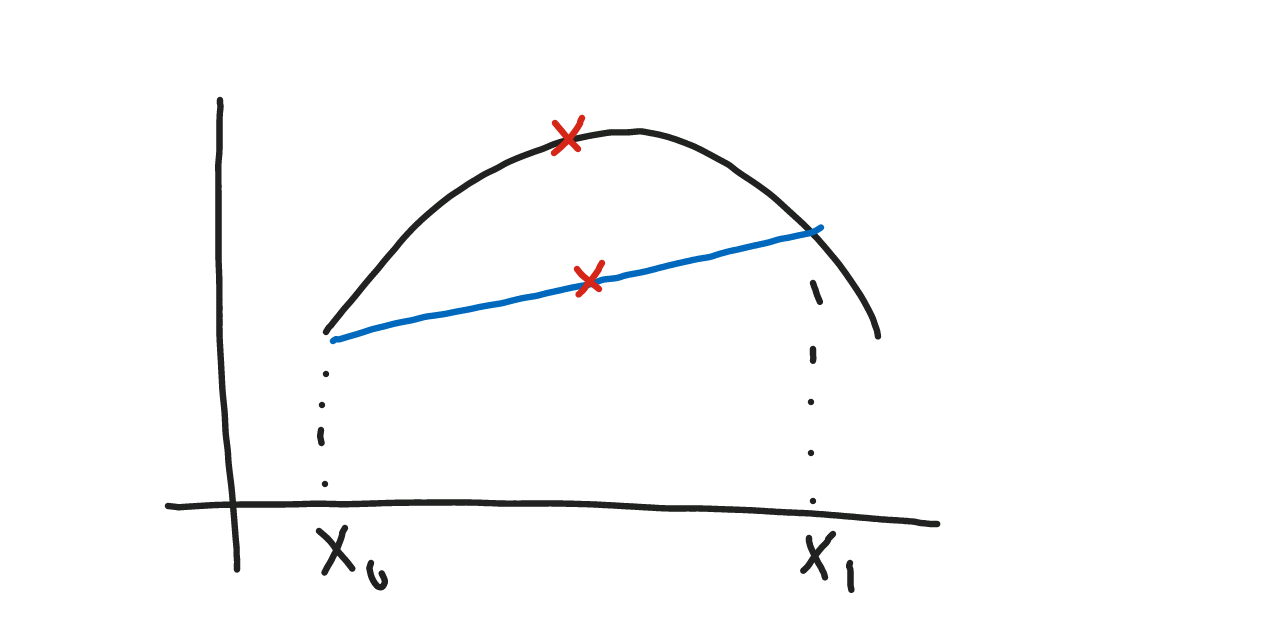
\includegraphics[scale=.25]{images/3-1}\end{center}

\begin{proof}
Let $\left\langle {X}\right\rangle = \int X\rho(dx)$. Take any tangent to $F$ at $\left\langle {X}\right\rangle$. 
Note that $F$ may not be differentiable, so take the line to have slope $F'(\left\langle {X}\right\rangle+0)$.
%Note that $F$ may not be differentiable, so by this we mean take a line passing through $(\an{X},F(\an{X}))$ with slope
%\be
%F'(\an{X}+0) \le \mu \le F'(\an{X}-0).
%\ee
%Then for all $x$, $F(x)$
The first inequality~\eqref{eq:jensen1} follows from concavity.
\begin{center}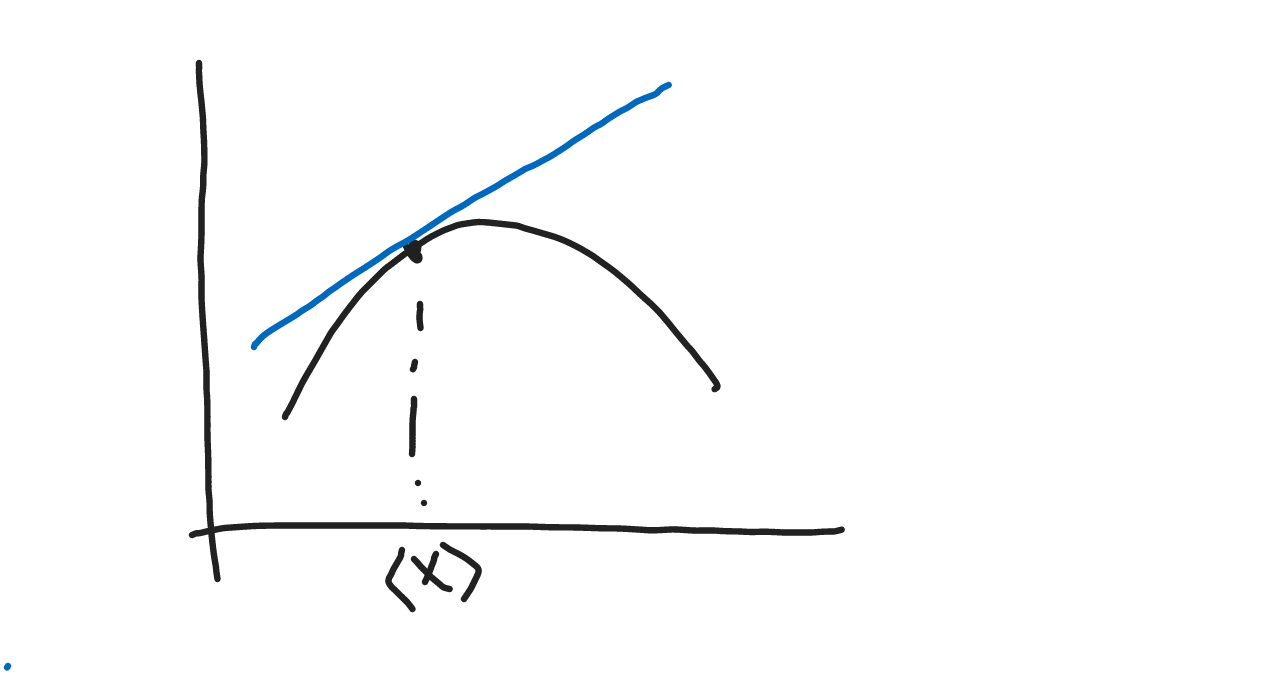
\includegraphics[scale=.25]{images/3-2}\end{center}
Integrate and note that $F(\left\langle {X}\right\rangle)$ is constant to get~\eqref{eq:jensen2}.
\begin{align}
\label{eq:jensen1}\text{{\color{red}\tiny eq:jensen1}}
F(X) &\le F(\left\langle {X}\right\rangle) + (X-\left\langle {X}\right\rangle) F'(\left\langle {X}\right\rangle+0)\\
\label{eq:jensen2}\text{{\color{red}\tiny eq:jensen2}}
\int F(X)\rho(dx)& \le \underbrace{F(\left\langle {X}\right\rangle)}_{\int \rho(dx)=1} + \underbrace{0}_{\int [X-\left\langle {X}\right\rangle]\,\rho(dx)=0}.
\end{align}
\end{proof}
This theorem is elementary but very useful. 

\section{Basic setup for statistical mechanics}
%The basic setup for statistical mechanics is as follows. 

The basic setup consists of... 

\begin{enumerate}
\item
A \textbf{lattice or a homogeneous graph} like $\mathbb{Z}^d$. %Often I'll use this as an example.
It will be important that for $\Lambda_L=[-L,L]^d$, 
\begin{equation}\label{eq:bdary-ratio}\text{{\color{red}\tiny eq:bdary-ratio}}
\frac{|\partial \Lambda_L|}{|\Lambda_L|} \xrightarrow{L\to \infty} 0.
\end{equation}

Here $|\cdot|$ means the size in terms of number of points (it doesn't matter much how you count---e.g. whether you count just the points on the edge, or adjacent too, etc.). \eqref{eq:bdary-ration} says when you chop space into regions, the boundary plays a small role. This is good becase we should be talking about extensive quantities.
\item
\textbf{Collection of local variables} like $\{n_x\}$ taking values in 0, 1, or $\{\sigma_x\}$ taking values in $\pm1$, magnetizations, etc.
%magnetization, other value of interest
\item
An extensive \index{energy function}\textbf{energy function}, defined on finite subsets. 
%interesting things happen in the infinite limit.
%Associate energy with finite subsets. 
For example, 
\be
H_{\Lambda}(\sigma)=-\sum_{(x,y)\subset \Lambda, |x-y|\le r}%\int_{x-y} 
\sigma_x\sigma_y - h\sum_{x\in \Lambda} \sigma_x.
%HL: not sure about this.
\ee
This is over a finite range; we can also consider unbounded ranges with some decay.

Here there are only pairwise interactions, but more generally, there can be interactions between more variables: 3, 4... Typically the interactions are translation invariant. The general equation is
\be
H_{\Lambda}(\sigma) = \sum_{A\subset \mathbb{Z}^d, \operatorname{diam}(A)\le R} K_A(\sigma),
\ee
where $K_A(\sigma)$ depends on $\sigma_{\upharpoonright A}$ ($\sigma$ restricted to $A$), and are shift covariant.

%finite range.
\item
%reference probability distribution.
A \textbf{reference a-priori (probability) measure} $\rho_0(d\sigma)$ (a probability distribution with respect to which we integrate) on the configuration space $\Omega_\Lambda$ ($=\{-1,+1\}^{\mathbb{Z}^d}$).

For example, $\rho_0(d\sigma)$ could be the product measure where $\{\sigma_x\}$ are iid variables. (Think of a system at high temperature.)\footnote{Note that it makes sense to talk about e.g. an infinite number of coin flips. There is such a thing as an infinite product of probability measures. In an infinite product space, the result of any finite collection is independent.  Any single value has probability 0.}\footnote{How does the Declaration of Independence go? ``We hold these truths to be self-evident... inalienable rights..." The definition of person is time-dependent. But there is a reference measure, individuals are treated equally. That's how we start in statistical mechanics. E.g. Every spin configuration gives equal value. If the spins are continuous, what would be a good starting point? Perhaps they are independently distributed on the sphere.}

We will also allow measures which are not probability measures---normalization may be ``part of the game."

Particle configurations are given by specifying locations and momenta. We can chop space into boxes, and specify the number of particles in each box, and their positions and momenta. The starting point is the Liouville measure, which is invariant under time evolution by the Hamiltonian.
\end{enumerate}

\subsection{Gibbs equilibrium measure}
\begin{definition}\label{df:gibbs-eq}\text{{\color{red}\tiny df:gibbs-eq}}
The finite-volume \index{Gibbs equilibrium measure}\textbf{Gibbs equilibrium measure} at temperature $T=\beta^{-1}$ is 
\begin{equation}\label{eq:gibbs-eq}\text{{\color{red}\tiny eq:gibbs-eq}}
\text{Prob}(d\sigma) = \frac{e^{-\beta H_{\Lambda}(\sigma)}}{Z_\Lambda} \rho_0(d\sigma_{\Lambda}).
\end{equation}
Here $Z_{\Lambda}$ is the normalizing (partition) function
\begin{equation}\label{eq:zla}\text{{\color{red}\tiny eq:zla}}
Z_{\Lambda}(\beta) = \int e^{-\beta H_\Lambda(\sigma_\Lambda)} \rho_0(d\sigma_A).
\end{equation}
\end{definition}
This is a \index{generating function}\textbf{generating function} because taking the derivatives we can learn about the distribution of the random variable.

The Gibbs equilibrium measure is the uniform measure %by tilting it with 
multiplied by the Gibbs factor. Here, $\beta$ is a factor corresponding to the inverse of the \index{temperature}\textbf{temperature}.

\begin{itemize}
\item
When $\beta=0$, local variables are independently distributed. We have chaos; all states are equally likely.
\item
When $\beta$ cranked up, i.e., temperature is lowered, the probability distribution becomes more concentrated (near the ``ground state"). When $\beta=\infty$, the distribution becomes concentrated on configurations which minimize the energy.
\end{itemize}•
We will see that the Gibbs equilibrium measure is the distribution of a system at thermal equilibrium at temperature $T$. Why is that so and what is the relation to microcanonical ensemble?

We will try to understand the structure of these measures and the phase transition they manifest.

\subsection{Introduction to the Ising model}

In biology, they study Drosophila, the fruit fly. Studying this simple organism tells us a lot.
The Ising model is the Drosophila of statistical physics. What you learn from it extrapolates to many other systems, but not everything.

%At low configurations, the configurations settle close to the ground state. 

Consider the \index{Ising model}\textbf{Ising model} on $\mathbb{Z}^d$,
\be
H_\Lambda(\sigma) = -\frac{1}{2}\sum_{|x-y|=1} J \sigma_x\sigma_y - h\sum_{x\in \Lambda} \sigma_x, \qquad J\ge 0.
\ee
At $T=0,\beta=\infty$, the state with all $+$'s and the state with all $-$'s are equally likely.
There is no continuous way to go from all spins $+$ to all spins $-$.
%analytic in finite volume may have nonanalytic limits.
%Nontrivial statement that the Gibbs function is analytic in $x$ for $h$ nonzero. Another statement, one of the general things you learn in statistical mechanics, is that for $H=0$ this is an analytic function even after you take the infinite limit. 
For nonzero, analytic even after take infinite limit.


However, the analyticity would fail, and in fact you would find a line of first order transitions at $H=0$ up to some temperature $T_c$. 
What happens is a natural extension at zero temperature and infinite $\beta$. You go from configuration that is all $+$ to all $-$ going through a discontinuity. 
The Gibbs state---the trivial distribution at this temperature---comes in 2 flavors (at least, other possibilities can hold): The state would remember whether the magnetic field $H$ was turned to 0 from the positive or negative side. This is a beautiful example of what you observe in magnets. 

The floor under the Atlantic ocean has ferromagnetic rocks. It was detected that the direction of magnetization changes. When you cool a ferromagnet (ferromagnets develops magnetic moments), which way it points is affected by the prevalent external field. According to prevailing wisdom, as the sea floor was expanding, the Earth's magnetic moment flipped. The rocks have encoded in them the direction of magnetization when they were cooled past this critical temperature. This phenomenon is called residual magnetization.
%There is a phenomenon of residual magnetization which remembers how it got to this state.. 
This phenomenon is eliminated when you raise to high enough temperature; then the state becomes the analytic. 
%infinite volume measure. 
We will discuss more about this phase transition, including behavior near the critical point, later.

This refers to the infinite volume limit of such measures. In finite volume, everything is analytic. 
At 0 temperature the configuration is all $+$, but at small temperature, thermal fluctuations occur. Unlike when $\beta=\infty$, when $\beta$ is finite, every local configuration gets some nonzero weight. Even thoguht there is a preference for agreement, the system exhibits fluctuations. Among the $+$'s there will be islands of minority spins. As temperature increase, minority fluctutions increase to a point where each spin tries to agree both with its neighbors and with magnetic field. When there is a lot of fluctuation among its neighbors, the effect of magnetic field is not so significant. That's how this discontinuity evaporates when you increase temperature.

\subsection{Entropy, energy, and free energy}
\begin{definition}
Let $\rho_0$ be a reference measure.
\begin{enumerate}
\item
For any probability measure $\mu$ on $\Omega_{\Lambda}$\footnote{that is absolutely continuous with respect to $\rho_0$}, we can write it in terms of $\rho_0$,
\be
\mu(d\sigma_\Lambda) = g(\sigma) \rho_0(d\sigma_\Lambda).
%ratio of the measures
\ee
The function $g(\sigma)$, the ``ratio" of the measures, is called the \index{Radon-Nikodym derivative}\textbf{Radon-Nikodym derivative}, and denoted by
\be
g(\sigma) = \frac{\delta\mu}{\delta\rho_0}.
\ee
%trace of density times log of density.
%canonical symbol is Radon-Nikodym derivative.
\item
Define the \textbf{entropy} of $\mu$ as
\be
S_\Lambda(\mu|\rho_0) = -\int g(\sigma_\Lambda)\ln g(\sigma_\Lambda) \rho_0(d\sigma_\Lambda).
\ee
\item Define the \index{energy content}\textbf{energy content} of $\mu$ as 
\be
E(\mu) = \int H_{\Lambda}(\sigma_{\Lambda}) \underbrace{g(\sigma_{\Lambda})\rho_0 (d\sigma_\Lambda)}_{\mu(d\sigma_A)}.
\ee

\end{enumerate}•
\end{definition}
%expected value of energy with respect to measure, entropy
\begin{theorem}\label{thm:gibbs-eq}\text{{\color{red}\tiny thm:gibbs-eq}}
For each $\beta\in [0,\infty)$, the Gibbs equilibrium measure~\eqref{eq:gibbs-eq} is the unique minimizer of 
\be
\beta F_\Lambda(\mu) := \beta E_{\Lambda}(\mu) - S_\Lambda(\mu|\rho_0),
\ee
equivalently, the unique maximizer of $S_{\Lambda}(\mu|\rho_0) - \beta E_{\Lambda}(\mu)$.
%negative temperature?
\end{theorem}
\begin{definition}
The quantity $\beta F_{\Lambda}(\mu)$ is called the \textbf{free energy}.
\end{definition}
We'll keep $\beta$ positive, but we can make sense of some of the theory when $\beta$ is negative. Sometimes we can even talk about $\beta$ complex!
%temperature is positive, otherwise call a doctor.

The second law of thermodynamics says that nature ``maximizes entropy under constraints." %Except at the thermal size, 
Here we're maximizing entropy minus energy. How to reconcile this? 
%it's constrainted in the microcanonical ensemble, not constrained in the grand canonical ensemble. 
There is some reservoir where the system trades with the entropy. As it trades off energy with the reservoir, the energy of the reservoir is affected. It is the effect of the entropy of the reservoir that the system has energy $E$. What the system is really maximizing is the entropy of the \emph{system and reservoir}.
%nice to think in terms of entropy

The free energy $\beta F_{\Lambda}(\mu)$ is the energy you get from the system when in thermal contact.\footnote{It's funny to talk about the energy crisis: we never run out of energy. The problem is that we have too little \emph{free} energy, we have too much entropy.}

%\begin{proof}[Proof of Theorem~\ref{thm:gibbs-eq}]
%Let $\rh_\be (d\si) = e^{-\be  H_\La(\si)}{Z_\La(\Ga)} \rh_0(d\si)$. Let $\psi(x)=-x\ln x$  which looks like the following.
%\ig{images/3-3}{.1}
%We bound the entropy using Jensen's inequality with $X= \fc{\de\mu}{\de \rh_\be}$,
%\bal
%S(\mu|\rh_0)&=-\int \fc{\de\mu}{\de\rh_\be} \ln \pf{\de\mu}{\de\rh_\be} \,\rh_\be (d\si_\La)\\
%& =\int \psi\pa{\fc{\de\mu}{\de\rh_\be}(\si_\La)}\rh_\be(d\si_\La)\\
%& \le \psi\pa{\an{\fc{\de\mu}{\de\rh_\be}}}=\psi(1)=0
%\end{align*}
%%average of concave function is below function at the midpoint
%%using $\an{X} = \int \fc{\de\mu}{\de \rh_\be}$, $\int \mu(d\si_\La)=1$, with 
%Equality holds if and only if 
%\be
%\fc{\de\mu}{\de\rh_\be} = \an{\fc{\de\mu}{\de\rh_\be} }= 1
%%evaluate what this means you end up with this expression.
%\ee
%where 
%\be
%\fc{\de\mu}{\de\rh_\be} = \fc{\de \mu}{\de \rh_0} \fc{Z_\La(\be)}{e^{-\be H_\la(\be)}}
%\stackrel{\text{claim}}= S(\La)(\mu|\rh_0)-\be E_{\La}(\mu).
%\ee
%%take the log
%To see the claim, note that the LHS is
%\bal
%&=\int \fc{\de\mu}{\de\rh_\be} \ln \pf{\de\mu}{\de\rh_0} \rh_\be(d\si)
%+ \ln Z_\La(\be) \ub{\int \fc{\de\mu}{\de\rh_\be}\rh_\be(d\si)}{=1} - \be \ub{\int \fc{\de\mu}{\de\rh_\be}H_{\La}(\si) \rh_\be (d\si)}{H_\La(\si) \mu(d\si_\La)}
%%energy function, last \de/\de. same as 
%%changes of notation, need experience.
%\end{align*}
%\fixme{This isn't quite right. I will post a complete derivation later. Change of variables?}
%\end{proof}
%By Jensen's inequality, the entropy is maximized when $S_{\La}(\mu|\rh_c)$. %, so it's uniquely maximized when equal to thermal state. 

What is the consequence? The thermal states are the states which maximize the difference. This allows to quantify the difference. When $\beta$ is small, the energy plays a minor role. The states maximize the entropy. As the temperature descreases and $\beta$ increases, $\beta E_\Lambda(\mu)$ in the variational principle plays an increasing role; the energy has to be low; $\beta$ controls how low it has to be. 

What's coming next? We'll pay attention to the factor $\ln Z_\Lambda(\beta)$. (Recall $Z_\Lambda(\beta)$ was defined in~\eqref{eq:zla}.) We will calculate 
\be\lim_{\Lambda \nearrow\mathbb{Z}^d} \frac{1}{|\Lambda_L|} \ln Z_{\Lambda}(\beta).\ee
%This ($S-\be E$) would be
%\be
%Z_{\La}(\be) = \int e^{-\be H_\La(\si)} \rh_0(\de).
%\ee
The relevant contribution comes only from configurations which are at an energy where the entropy is maximized. 

Entropy appears in many guises. We talked about entropy over a measure, but you can also talk about the entropy function of energy; the contribution from those particles would be $e^{S(E)}e^{-\beta E}$. Now it's just a function of the energy. This function picks up the Legendre transform of the entropy.
%It picks up the Legendre transform... as a function of energy. 

 %the contribution comes is $e^{-\

In the Ising model, there is a discontinuity in the nature of the states. Differentiability of the free energy function breaks down across the line. There is an interplay between convexity properties of thermodynamic functions. The left and right derivative---the mean values of the magnetization---corresponds to 2 different limiting values, that are the two different magnetizations depending on which way you arrive. %Concave functions of parameters.

Statistical mechanics translates into the nonuniqueness of Gibbs equilibriums state. Statistical mechanics provides much more information because it looks at the joint distribution of all these variables, whereas thermodynamics just fixes attention on a few relevant parameters. We will clarify this relation. 
We will clarify this and then discuss techniques to find the phase transitions.
%\section{A variational characterization of Gibbs States} 

%\section{First order phase transitions}

